% !TEX root = ../main_zh.tex
\chapter{货币、银行与货币政策}
\label{ch:money}

到目前为止，宏观经济学里我们研究过的几乎一切——产出、资本、劳动、增长——原则上都可以在完全不提“货币”的情况下讲清楚。第~\ref{ch:solow}~章和第~\ref{ch:neoclassical}~章的索洛模型与新古典模型，整套都是用实际产品来书写的。然而，没有任何一个现代经济体能离开货币运转；而政府在短期内为管理宏观经济所\emph{真正做}的事，绝大部分都是通过中央银行来完成的。本章讲的就是这套“管道系统”：货币是什么，银行体系如何制造出其中的大部分，以及中央银行用哪些工具来扩张或收缩信贷供给。

这个主题不可避免地比之前的模型更偏制度性。凡是有干净结构的地方——资产的流动性排序、货币乘数、央行资产负债表——我们都会把它精确地讲出来。但货币政策的很大一部分，是“谁、通过哪种法律工具、对谁、做了什么”的问题，而这些安排在各国之间差异极大。本章贯穿始终的两个参照体系是：美国，其央行主要通过国债市场运作；中国，其央行主要直接通过商业银行运作。我们会比较细致地处理中国特有的这套机制，一来因为课程如此，二来因为它更清晰地展示了一家央行如何借助银行渠道来驾驭一个经济体。除非另有说明，下文中的“央行”指的都是中国人民银行（PBoC）。

有两个看似该放在本章的主题，被安排到了别处。消费者价格指数和生产者价格指数（CPI 与 PPI），即我们对价格水平的度量，已在第~\ref{ch:prices}~章建立。货币数量论、通胀税与铸币税——这些是\emph{印}钞所带来的后果，而非\emph{管理}货币的机制——则是第~\ref{ch:quantity}~章的内容。这里我们只谈制度。

\section{货币与流动性}

理解货币最好的方式，是把它看作一种\emph{资产}——一件可以持有的、有价值的东西——它与其他资产的区别，首要在于一项性质：流动性。一项资产的流动性，指的是它能在多大程度上被又快、又便宜、又以可预期的价值兑换成商品。手中的现金是这条谱系的极端情形：它处处被接受、即时生效、按面值兑付。一张政府债券、一份共同基金份额或一只上市股票同样是价值储藏，但要把它变成可花的购买力，需要时间，而且可能被迫在不利价位上卖出。货币的定义性特征，就是它处在这条流动性谱系的高流动性一端。

让一项资产被接受为货币的，归根结底是\emph{信用}（credibility）：人们之所以肯收下它来交换，只是因为他们确信别人也会再从自己手里收下它。这种接受面越广，资产的流动性就越高。图~\ref{fig:macro-10}把主要的金融资产沿这一维度排了序。

\begin{figure}[h]
\centering
\begin{tikzpicture}[font=\small]
  % --- geometry of the spectrum ---
  \def\W{14.0}        % total width of the arrow body
  \def\H{1.4}         % half-height of the arrow body
  \def\head{1.6}      % horizontal length of the arrowhead
  \def\tip{2.05}      % half-height at the base of the arrowhead

  % wide right-pointing arrow (least liquid on the left, most liquid on the right)
  \draw[line width=0.8pt, rounded corners=2pt, fill=black!6]
        (0,\H) -- (\W,\H) -- (\W,\tip)
        -- (\W+\head,0)
        -- (\W,-\tip) -- (\W,-\H) -- (0,-\H) -- cycle;

  % --- four rounded boxes inside the arrow, left to right ---
  \tikzset{libox/.style={draw, line width=0.8pt, rounded corners=5pt,
                         minimum height=1.55cm, align=center,
                         inner sep=4pt, anchor=center}}

  \node[libox, minimum width=2.95cm] (b1) at (1.85,0)
        {Government bonds,\\ funds, stocks};
  \node[libox, minimum width=2.45cm] (b2) at (5.35,0)
        {Time deposits};
  \node[libox, minimum width=4.0cm] (b3) at (9.3,0)
        {Checks,\\ demand deposits};
  \node[libox, minimum width=1.75cm] (b4) at (12.85,0)
        {Cash};

  % --- caption beneath: increasing liquidity ---
  \draw[-Latex, line width=0.9pt] (0,-2.55) -- (\W+\head,-2.55);
  \node[below, anchor=north] at ({(\W+\head)/2},-2.62) {increasing liquidity};
\end{tikzpicture}

\caption{流动性谱系：从最左端流动性最低的资产（债券、基金份额、股票），到最右端流动性最高的资产——现金。}
\label{fig:macro-10}
\end{figure}

\defn{流动性}{
一项资产的\emph{流动性}（liquidity），是指它能在不损失价值的前提下被转换为普遍接受的支付手段的难易程度。货币按定义就是流动性最高的一类资产；而现金是货币中流动性最高的形态。
}

一个有用的推论是：流动性是被定价的。一项流动性较低的资产，必须提供一个\emph{溢价}（premium）——更高的预期收益，或一个价格折让——才能与流动性更高的资产并存被人持有；否则没人愿意忍受持有它的不便。“低流动性资产相对高流动性资产折价交易”这一条想法，本身就组织起了银行体系与央行所做的大部分事情。

\begin{remark}[银行业即一场流动性转换]
银行贷款是有抵押的：借款人质押一项低流动性资产（一套房子、一只债券、一座工厂），换回高流动性的资金。借款人那笔不易变现的财富，实际上被换成了流动的购买力，而即便没有任何新的实物资产被创造出来，实体经济可动用的\emph{总}流动性也上升了。央行在更上一层做的是完全相同的事：它以政府债券等抵押品向商业银行放款，把银行那些流动性较低的持有物，换成流动性最高的那种资产。调控全社会的流动性，正是央行日常的本职工作。比如，当财政部征税时，它是在从私人部门抽走流动性；央行通常会对应投放基础货币来对冲，使这一轮征税不会造成一次意料之外的货币紧缩。
\end{remark}

\section{货币层次}

由于“货币”涵盖了流动性各异的资产，统计部门并不会用单独一个数字来报告它。它们报告的是一族嵌套的\emph{货币层次}（货币总量，monetary aggregates），每一层都在里一层之上，再添上一层流动性更低、更像存款的工具。图~\ref{fig:macro-11}展示了标准的嵌套关系，$M_0 \subset M_1 \subset M_2$。

\begin{figure}[h]
\centering
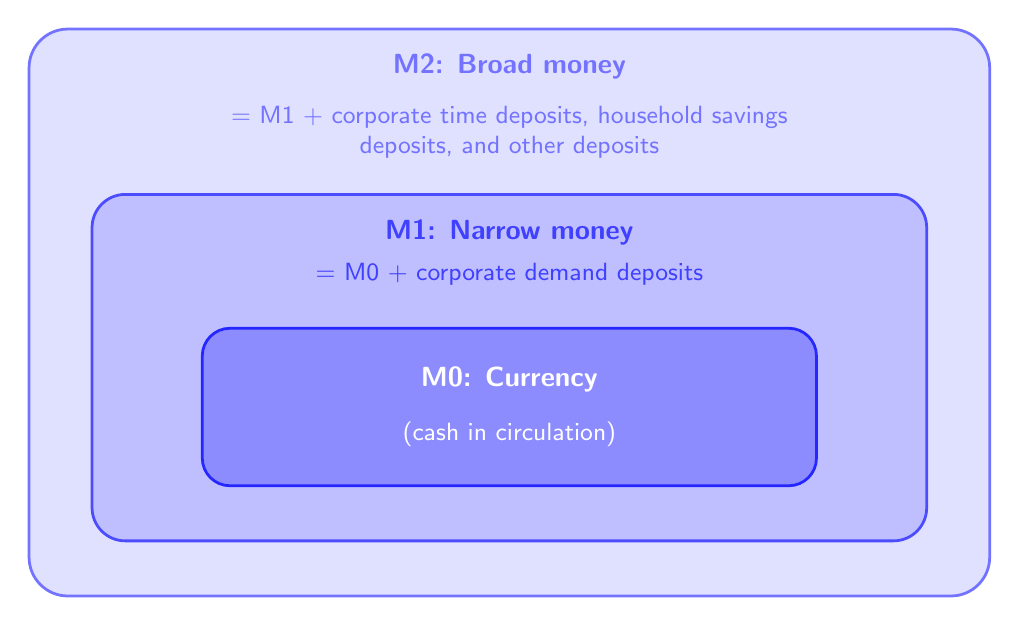
\begin{tikzpicture}[font=\sffamily]
  % Monetary aggregates as TRUE nested containment: M2 contains M1 contains M0.
  % Graduated blue shades convey the subset relation M2 \supset M1 \supset M0:
  % outermost lightest (M2), middle (M1), innermost darkest (M0).

  % --- M2: outer, lightest box (broad money) ---
  \draw[fill=blue!12, draw=blue!55, line width=1pt, rounded corners=14pt]
    (0,0) rectangle (12.2,7.2);
  \node[anchor=north, font=\sffamily\bfseries, text=blue!55] at (6.1,7.0)
    {M2: Broad money};
  \node[anchor=north, align=center, text width=11.6cm, font=\sffamily\small,
        text=blue!55] at (6.1,6.35)
    {$=$ M1 $+$ corporate time deposits, household savings\\
     deposits, and other deposits};

  % --- M1: middle box, lighter shade (narrow money) ---
  \draw[fill=blue!25, draw=blue!70, line width=1pt, rounded corners=12pt]
    (0.8,0.7) rectangle (11.4,5.1);
  \node[anchor=north, font=\sffamily\bfseries, text=blue!75] at (6.1,4.9)
    {M1: Narrow money};
  \node[anchor=north, align=center, text width=9.8cm, font=\sffamily\small,
        text=blue!75] at (6.1,4.35)
    {$=$ M0 $+$ corporate demand deposits};

  % --- M0: inner box, darkest shade (currency) ---
  \draw[fill=blue!45, draw=blue!85, line width=1pt, rounded corners=10pt]
    (2.2,1.4) rectangle (10.0,3.4);
  \node[font=\sffamily\bfseries, text=white] at (6.1,2.75)
    {M0: Currency};
  \node[align=center, text width=7.0cm, font=\sffamily\small, text=white]
    at (6.1,2.05)
    {(cash in circulation)};
\end{tikzpicture}

\caption{嵌套的货币层次：通货 $M_0$ 套在狭义货币 $M_1$ 之内，而 $M_1$ 又套在广义货币 $M_2$ 之内。}
\label{fig:macro-11}
\end{figure}

\defn{货币层次}{
货币层次按流动性把货币排序：
\begin{itemize}
    \item $M_0$ —— 流通中的通货：处在银行体系之外的实物现金，是流动性最高的部分。
    \item $M_1$ —— “狭义货币”：$M_0$ 加上活期（可开支票的）存款，这类存款能在短时间内动用。
    \item $M_2$ —— “广义货币”：$M_1$ 加上定期存款与储蓄存款，这类存款流动性略低。
\end{itemize}
每一层都严格包含它里面的各层。
}

通货部分 $M_0$ 规模很小，主要受短期、季节性因素（节假日、发薪周期）驱动。对政策真正重要的层次是 $M_2$。现金只占 $M_2$ 中很小的一部分；现代经济中绝大部分“货币”根本不是纸钞，而是\emph{存款余额}——银行账面上的记账。一句话说：货币就是账面上的钱。

\begin{remark}[持有的货币与社会上的货币]
$M_0$、$M_1$、$M_2$ 度量的都是公众\emph{实际持有}的货币。这既不等同于整个体系所\emph{能}创造出的货币总量，也不等同于“财富”。这些层次量度的是某一时点上流通中的流动性债权存量，仅此而已；不要把它们读作经济中全部购买力的一次普查。
\end{remark}

\subsection{为何 \texorpdfstring{$M_2$}{M2} 是政策目标}

$M_2$ 是观察货币增长的主视角。$M_2$ 的\emph{增速}是货币政策的头条度量；在中国，每年“两会”常把这一目标定在大约百分之十。作为经验法则，$M_2$ 的增速被期望与名义 GDP 的增速大体匹配——新增的货币恰好够为新增的交易融资，不多不少。但严格说来，这条规则不可能机械地成立，因为货币政策的全部要义恰在于\emph{逆周期}：央行会刻意让货币在衰退期增长得快于产出、在繁荣期增长得慢于产出。一个每季度都简单地跟住名义 GDP 的货币供给，根本就没在做任何稳定经济的工作。

\begin{remark}[$M_2/\mathrm{GDP}$ 之比很容易被误读]
中国的 $M_2$ 与 GDP 之比超过 200\%，而美国的不到 100\%。人们很容易由此断定中国流动性泛滥、而美国没有。但这一比较并不支持这个结论，理由有好几条。

第一，两国央行的行事风格大不相同：中国人民银行在扩张货币供给上一向很收敛，而美联储则是大开大合（危机时大幅降息，事后再反向操作）。第二，也更根本的，是 $M_2$ 被创造出来的\emph{渠道}不同。在美国、英国这样的普通法经济体中，\emph{直接金融}占主导：企业主要靠发行债券和股票来筹钱，这些都不会穿过、也不会推高银行存款类的货币总量。中国则依赖\emph{间接金融}：企业向商业银行借款，而每一笔这样的贷款都会派生出一笔与之对应的存款，于是一个信贷驱动的经济体，机械地就会背负一个相对 GDP 更大的 $M_2$。商业银行是中国金融体系的中枢。第三，$M_2$ 是\emph{存量}，GDP 是\emph{流量}；二者之比混用了量纲，只有它们的\emph{增速}才可能被有意义地比较。最后，改革开放以来的快速市场化，把许多原本非市场化的活动逐步货币化了，这也出于与“过剩”无关的原因把 $M_2$ 推了上去。
\end{remark}

\subsection{贷款与社会融资}

$M_2$ 与银行信贷同涨同落，因为在间接金融体系中，新增贷款是新增广义货币的主要来源。除了 $M_2$ 的两大教科书驱动因素——基础货币的供给与货币乘数（在下一节展开）——之外，$M_2$ 增长还可能因\emph{需求}侧的原因而停滞：实体经济可能不想借（信贷需求疲弱），或者银行可能不愿放（“信贷紧缩”，银行囤积流动性）。因此，把两个相关的概念分开来谈是有用的。

\state{宽货币与宽信用}{
\emph{宽货币}（“货币宽松”立场）指的是央行增加基础货币的供给。\emph{宽信用}（“信用宽松”立场）指的是实体经济确实更容易获得融资了——信贷的可得性变宽了。二者并不是一回事：如果宽货币没能转化为宽信用，那就说明\emph{货币传导机制}受阻，多投放的基础货币会淤积在银行体系里，到不了企业和居民手中。
}

有几个公开发布的数据序列，能让分析者直接观察信贷渠道。\emph{人民币新增贷款}是观测间接金融的关键指标，分为住户贷款与企业贷款两块。住户贷款以消费贷为主；近年来消费贷与信用卡余额的违约率急剧上升。一个更宽口径的度量是\emph{社会融资规模}。

\defn{社会融资规模}{
\emph{社会融资规模}度量的是金融机构向实体经济——向企业与个人——提供的全部融资，并\emph{不包括}金融机构彼此之间的借贷。它既涵盖通过银行体系的间接融资（贷款、信托贷款、未贴现银行承兑汇票——后两者属于“表外”），也涵盖通过资本市场的直接融资（债券与股票）。普通的银行贷款记为“表内”；信托贷款与委托贷款记为“表外”。
}

市场尤其紧盯三个头条数字——$M_2$、人民币新增贷款、社会融资规模——通常在每月的 10 日至 15 日之间公布。

\section{货币的类型}

货币说到底，是一个社会共同同意去讲的一个故事。是什么赋予某个特定物件以货币价值，这在历史上一直在变，而这些差异本身很有启发性。

\paragraph{商品货币。}商品货币有内在价值：物件本身就值点东西（黄金、白银、铜），所以它的货币价值锚定在它的材料价值上。因此，商品货币的供给量由生产技术决定——比如能开采出多少白银——无法随意扩张。

\begin{remark}[纸币比你想的要古老]
2022 年是\emph{交子}问世一千周年，交子是中国早期的一种纸币。中国长期受困于贵金属稀缺，古代大多使用铜钱，白银很少；宋朝甚至试用过铁钱，其一大弊病是会生锈。纸币的早早出现本身就是一个信号：它恰恰出现在商业活动已经活跃到现有的贵金属存量不足以结清所有交易的时候。纸币正是对流动性短缺的一种回应。
\end{remark}

\paragraph{法定货币。}法定货币没有内在价值——一张钞票不过是印了字的纸——它被接受的原因有二。其一是\emph{发行者的信用}：发行机构可信到足以让它的票据流通（历史上，那些声誉极高的私人银行的票据）。其二，也是现代货币的根基，是\emph{国家的信用}：主权力量强制其被接受，票据由央行发行。央行甚至可以把发行权委托给指定的、可靠的商业银行——香港没有央行，其货币就由发钞银行发行。

流通中的现金是央行的\emph{负债}，是持有者的\emph{资产}——这一点我们待会儿读央行资产负债表时会用到。布雷顿森林体系瓦解以来，货币就成了纯粹的法定（信用）货币，不再可以兑换成黄金。

\state{信用货币可以随意创造}{
商品货币的供给由生产能力（白银的开采速度）固定。法定（信用）货币的供给则是人的决定：它基本可以无限制地扩张，而一个信用货币体系只要国家的信用还在，就能维系。一旦那份信用崩塌——公众不再信任本币、转而投奔外币——结果就是恶性通货膨胀。所以这种对货币“透支”的余地虽是真实的，却被信心所限。
}

\paragraph{数字货币与加密货币。}一种加密货币是被私下认可的货币，其供给由算法固定。由于供给固定、而物件本身又一文不值，它的价格波动极大。它的定义性特征是\emph{供给固定}与\emph{去中心化}——没有央行——而不在于它仅仅是“数字的”（电子支付与线上转账同样是数字的，但那些是对普通银行存款的债权）。在这一点上，比特币很像黄金：黄金本身不带来任何收益，唯一的回报就是其价格的变动，这正是为什么二者都是投机的对象，而不像股票或债券那样是会产生收入的投资。这类资产把价值储藏功能与交易功能结合在一起，因而带有一定的价值；而在地缘政治风险加剧的世界里，这种价值还可能增长。

\section{货币传导机制}

一项央行行动是如何抵达一个普通借款人的？答案——\emph{传导机制}——在不同国家要经过不同的中间市场。

\begin{center}
\renewcommand{\arraystretch}{1.4}
\begin{tabular}{@{}ll@{}}
\toprule
& 传导链条 \\
\midrule
中国 & 央行 $\to$ \textbf{商业银行} $\to$ 社会 \\
美国 & 央行 $\to$ \textbf{国债市场} $\to$ 社会 \\
\bottomrule
\end{tabular}
\end{center}

这一对比，恰恰就是前面那个直接金融与间接金融的区别。在美国，央行作用于国债市场——一条直接金融渠道——其余的经济部门再根据国债收益率重新定价。在中国，央行作用于商业银行——一条间接金融渠道——银行再把这一脉冲传递给企业和居民。

美国的这条渠道立足于一条资产负债表恒等式。\emph{国债是央行的资产，现金是央行的负债。}当美联储\emph{买入}债券时，它的资产负债表\emph{扩张}，并用新创造的货币来支付债券价款，从而抬高货币供给。当它\emph{卖出}债券时，资产负债表\emph{收缩}，货币被从流通中抽走。所以买债即放松、卖债即收紧。美国国债市场的主要交易对手本身也是商业银行；其独特之处在于美联储是作为又一个普通交易方平等地参与买卖，而非直接向银行放款。由于现金只占 $M_2$ 中很小的份额，央行里最重要的部门并不是负责现金发行的，而是执行这些市场操作的货币政策司。

\section{准备金制度与货币乘数}

现在我们触及现代银行业的那个核心机械事实：\emph{创造出大部分货币的，是商业银行，而不是央行。}它们靠准备金制度来做到这一点。一家银行收到一笔存款，只被要求把其中一小部分作为\emph{准备金}留下，余下的可以放贷出去；这笔贷款会在别处变成一笔存款，又被大体放贷出去，如此往复。一单位基础货币撑起的是其若干倍的存款。乘数量化的就是这个“若干倍”。

\defn{货币乘数}{
记 $C$ 为公众持有的通货，$D$ 为存款，$R$ 为银行准备金。广义货币为 $M = C + D$，而\emph{基础货币}（也称\emph{高能货币}）为 $B = C + R$。\emph{货币乘数}就是下面这个比值
\[
\text{货币乘数} \;=\; \frac{M}{B} \;=\; \frac{C + D}{C + R}
\;=\; \frac{c + 1}{c + r},
\]
其中 $c = C/D$ 是\emph{通货存款比}，$r = R/D$ 是\emph{准备金率}。第二个等号是把分子分母同除以 $D$ 得到的。
}

这个推导值得做一遍，因为代数本身就是全部内容所在。从 $M = C + D$ 与 $B = C + R$ 出发，把 $M/B$ 的分子分母同除以存款 $D$：
\[
\frac{M}{B} \;=\; \frac{C/D + D/D}{C/D + R/D} \;=\; \frac{c + 1}{c + r}.
\]
这个表达式的两个特征承载了全部经济学含义。第一，通货 $C$ 是从银行体系里\emph{漏出去}的货币；它躺在钱包里，无法被再次放贷，所以通货存款比 $c$ 越高，乘数就越小。实践中 $c$ 很小，因为公众持有的现金相对存款而言很少。第二，也是那个政策杠杆，就是准备金率。

\thm{准备金率越低，乘数越高}{
保持通货存款比 $c$ 不变，货币乘数 $\dfrac{c+1}{c+r}$ 关于准备金率 $r$ 严格递减。$r$ 越低，银行就能把每笔存款中更大的比例放贷出去，从而支撑起更多轮的存款派生，于是从同样的基础货币里生成更大的 $M_2$。
}
\pf{
将 $m(r) = (c+1)/(c+r)$ 关于 $r$ 求导：
\[
\dd{m}{r} = -\frac{c+1}{(c+r)^2} < 0,
\]
因为 $c+1 > 0$。故 $m$ 随 $r$ 上升而下降、随 $r$ 下降而上升。
}

这正是为什么法定准备金率是一项货币政策工具：在基础货币不变的情况下下调它，会机械地抬高 $M_2$。而基础货币本身由央行供给。

\defn{基础货币}{
\emph{基础货币}（高能货币）是央行直接创造出来的货币——“最初的钱”。在间接金融体系里，它在央行向商业银行放款时进入经济。央行向银行释放的一切资金都是基础货币。由于它随后会被货币乘数放大，基础货币会生成一个远大于其自身的 $M_2$。因此，$M_2$ 的增长主要来自两个来源：基础货币的供给与准备金率。
}

\subsection{银行为何会把准备金压得过低：道德风险与准备金红线}

准备金是在安全与利润之间做权衡。持有更多准备金的银行更安全、但赚得更少，因为闲置的准备金几乎不生息；持有更少准备金的银行赚得更多、但更容易遭遇挤兑。每家银行只在意自己的利润，而利润是私有的、排他的。然而，安全却带有\emph{外部性}：一家银行的倒闭可能在整个体系中层层传染。由于知道金融体系会动员起来救助某个陷入困境的成员，每家银行都有动机搭便车——把自己的准备金率压得更低、攫取那份利润，而让系统性的安全由别人来提供。这是一个经典的\emph{道德风险}（moral hazard），它还会孳生逆向选择：在没有管制的情况下，活下来的银行恰恰是风险最高的那些，因为它们赚得比稳健的同行多。

\begin{remark}[准备金红线即一条互助规则]
制度上的应对，是一条协调一致的准备金\emph{红线}。各家银行实际上结成了一个带有红线的互助会：如果某个成员陷入困境时，其准备金水平\emph{高于}红线，互助会就有义务去救它；若其准备金\emph{低于}红线，则不予救助。这条红线恢复了持有足额准备金的激励。历史上，央行所扮演的正是这个最后贷款人、协调救助的角色，它由各成员银行所有，就像一个俱乐部或行业协会。比如美联储就是有股东的——那些成员银行——它把大部分利润上缴财政部、并分一部分给那些股东；然而无论是股东还是总统都无权指挥它的操作。一家现代央行立足的是国家的信用，而不是它的所有权。
\end{remark}

\section{中央银行}

央行本身也是一家银行，但它不以盈利为目的——尽管它在现实中盈利能力极强。它只与商业银行（以及少数指定机构）打交道，其利润来自\emph{利差}，主要是它就准备金支付的利率与它从放贷便利中所赚的更高利率之间的差（在中国，即准备金利率与 MLF 利率之间的利差）。

\begin{remark}[谁可以在央行开户]
只有银行和少数非银机构可以在央行开设账户。这里的“银行”包括商业银行与\emph{政策性银行}，后者中最重要的是国家开发银行（国开行）。政策性银行为基础设施这类规模大、利润薄、战略地位重要的项目提供资金；国开行可以自行发债（国开债），其资金最终由央行提供。中央财政部也可以开设账户——这相当于国库。央行还会指定一份\emph{一级交易商}名单，它们通常是在央行总部开户的大型商业银行；央行主要与这些一级交易商交易，再由它们向银行体系的其余部分转融通资金。
\end{remark}

由于央行不可能持续审查每家商业银行的现金，银行把准备金存放在\emph{设于}央行的准备金账户里，而准备金水平低于法定要求的银行会受到处罚。由于一家银行的存款时刻在波动，稳健的银行会在法定最低限之上多持有一些\emph{超额准备金}作为缓冲。央行会对超额准备金支付利息，但——为了防止银行仅靠把资金停泊在央行就获利——超额准备金利率不可能超过法定准备金利率，而且超额准备金事实上还设有上限。

\state{超额准备金利率是利率走廊的下限}{
超额准备金的利率确定了政策利率走廊的\emph{下限}：没有银行会以低于它在央行所能无风险赚到的利率去拆出隔夜资金。当超额准备金利率下降时，市场利率会随之下降。整个体系中较低的超额准备金率，意味着流动性吃紧——银行手头的闲钱很少。
}

\begin{remark}[央行代表谁的利益]
央行代表的是\emph{货币资产的持有者}——所有持有货币或类货币债权的人——而\emph{断然不}代表政府本身。当它放贷、把低流动性资产换成高流动性资产时，它服务的是这些债权人。它对独立性的坚持，恰恰是一种拒绝直接服务于政府融资需要的态度：一家被财政当局俘获的央行，只会去为政府赤字货币化。在中国，央行不可以直接\emph{购买}国债，但可以把国债作为\emph{抵押品}；而它发行的货币也不必与抵押品一一对应——它基本可以相机地创造信用货币。一些国家偏向于财政货币化，这一想法扎根于\emph{现代货币理论}（MMT，Modern Monetary Theory），该理论认为一个信用充足的主权国家，其货币发行的上限比通常想象的要高得多，而央行应当配合财政政策。中国人民银行强力捍卫自己的独立性，坚决反对财政货币化。
\end{remark}

\subsection{法定职责与组织结构}

简而言之，货币政策的运作，是通过设定三个工具——货币供应量、政策利率、准备金率——来驾驭三个目标：$M_2$、社会融资规模、人民币新增贷款。一家央行的法定职责框定了它要实现什么，而目标的排序很关键。

\state{中国人民银行的职责：币值稳定优先}{
中国人民银行是政府部门，在国务院的指导下制定和实施货币政策。它的目标是\emph{维持币值稳定，并以此促进经济增长}。币值稳定——也就是控制通货膨胀——是\emph{首要}目标；经济增长在其后。一条实务性的推论是：凡是收紧的，往往是央行自己发起的；而凡是宽松的，往往是政府向它施压促成的。
}

央行并不对经济增长直接负责；在中国，主管经济增长的牵头机构是国家发展和改革委员会，其次是财政部。央行对利率的调整也很谨慎：如果无风险利率定得太高，有风险的创业投资就会被挤得没有发展空间。

美国联邦储备体系尽管有私人股东，却行使着国家机构的职能。它的理事会总部设在华盛顿，由七名理事组成，而美联储主席的任期被刻意与总统任期错开。主席不是内阁成员，总统对美联储没有直接的行政命令权。

\defn{FOMC 与联邦基金利率}{
\emph{联邦公开市场委员会}（FOMC）制定美国的货币政策。它有 12 名投票委员：7 名理事，加上纽约联邦储备银行行长，再加上其余 11 位地区储备银行行长中轮值的 4 位（$7 + 1 + 4 = 12$）。它大约每六周开一次会。当美联储“加息”或“降息”时，它作用的是\emph{联邦基金利率}——美国各银行之间的隔夜同业拆借利率。
}

在市场化的体制下，美联储无法真的指定联邦基金利率；它宣布的是一个\emph{目标区间}。为了把实际利率维持在区间之内，它使用\emph{公开市场操作}来调节流动性，而这进一步会移动诸如十年期国债之类较长期工具的价格。实际上美联储很少直接向商业银行放款，也无法靠下令来固定大多数利率——它只能去引导一个区间。相比之下，中国的央行则与银行频繁交易，可以直接确定利率。

\begin{remark}[应对危机与对货币政策的过度依赖]
美联储应对危机的标准套路，是大幅降息、向体系灌入流动性，并接受其后的再通胀：2001 年互联网泡沫破裂与“9·11”之后、2008 年金融危机、以及 2020 年的疫情，都是这个模式。课程反复出现的一个主题是：西方经济越来越过度依赖货币政策，因为财政政策很难施展——像 2008 年之后的危机复苏，主要就是靠央行续命。一个治理上的对比把这一点讲得更尖锐：美国的货币政策由一个绝缘的技术官僚精英集团掌控，它快、但不民主；而对面是民主、却迟缓的国会。草根民主与精英专制之间的平衡在许多场合反复出现；危机当头时，美国只能通过这条快速的、技术官僚式的货币渠道来行动。
\end{remark}

\subsection{基于规则的政策与相机抉择的政策}

各国央行在可预测程度上各不相同。

\defn{基于规则的政策与相机抉择的政策}{
在\emph{基于规则}（rule-based）的政策下，央行遵循一条透明的、事先承诺好的规则，因而市场可以预判它的动作，央行也不会让预期落空。最典型的例子是\emph{泰勒规则}（Taylor rule），它把目标利率设为通胀与失业（或产出）缺口的函数。在\emph{相机抉择}（discretionary）的政策下，目标和工具被刻意保持模糊，因而市场无法对下一步动作形成精确预期。
}

美联储收紧的意图是公开摆明的——它大体遵循一条以通胀和失业为锚、经过优化的泰勒规则——这使得美国的政策是基于规则的。中国的政策目标则相对不透明，通过利率、准备金率、LPR 等一套工具来推进，这使得它是相机抉择的。

\begin{remark}[近年美联储周期的一条粗略时间线]
互联网泡沫破裂与“9·11”导致美国在 2001 年大幅降息，2005 年之后才恢复。2007 年的次贷危机迫使又一轮深度降息，并把利率长期维持在 0.25\% 附近。2017 年之后，经济充分恢复，美联储进入加息周期；2019 年，正值繁荣，特朗普总统却屡次强势要求降息。2022 年的加息比 2008 年之后那一轮更陡峭，并且是由市场\emph{两侧}共同驱动的：需求侧的经济复苏，以及供给侧的压力——劳动参与率下降，加上俄乌战争触发的能源价格飙升。如果通胀缓解，美联储可能会提前退出加息路径。
\end{remark}

\section{央行的资产负债表}

央行靠改变自身资产负债表的规模与构成来驾驭经济。会计账目是对它所作所为最干净的概括。

\state{如何读一张央行资产负债表}{
在央行的资产负债表上，\emph{流通中的现金是负债}，而\emph{债券（及其他买入的资产）是资产}。因此：\emph{扩表}——买入资产，并创造准备金和现金来支付——会向体系增添流动性，把利率\emph{往下}压；\emph{缩表}则抽走流动性，把利率\emph{往上}推。
}

下面是两张参照性的资产负债表，以 T 形账户呈现。

\begin{table}[h]
\centering
\begin{tabular}{@{}p{0.42\textwidth} p{0.42\textwidth}@{}}
\multicolumn{2}{c}{\textbf{美联储}}\\
\toprule
\multicolumn{1}{c}{资产} & \multicolumn{1}{c}{负债}\\
\midrule
债券（以国债与 MBS 为主） & 流通中现金（主要） \\
 & 银行准备金 \\
\bottomrule
\end{tabular}
\end{table}

\begin{remark}[MBS 是怎么进入美联储资产负债表的]
2008 年危机之后——其直接诱因是被打包成\emph{住房抵押贷款支持证券}（MBS）的次级债——美联储于 2009 年买入了大量 MBS 来救市。这正是为什么 MBS 会与国债并列，成为美联储资产负债表上的一项主要资产。
\end{remark}

\begin{table}[h]
\centering
\begin{tabular}{@{}p{0.42\textwidth} p{0.42\textwidth}@{}}
\multicolumn{2}{c}{\textbf{中国人民银行}}\\
\toprule
\multicolumn{1}{c}{资产} & \multicolumn{1}{c}{负债}\\
\midrule
外汇占款 & 流通中现金（主要） \\
债券 & 银行准备金 \\
\bottomrule
\end{tabular}
\end{table}

中国人民银行资产负债表上最醒目的特征，是资产侧那一大笔外汇占款，主要是为了维持金融体系的稳定而持有的。下面讲中国的政策工具箱时，我们会看到这些外汇占款的累积是如何在十多年里驱动了央行的资产负债表。

\section{常规与非常规工具}

除了设定准备金要求、开展市场操作之外，央行还备有一套梯度分明的工具，从例行的一直延伸到应急的。

\paragraph{贴现窗口。}除公开市场操作之外，美联储也会直接向金融机构放款；这就是\emph{贴现}，其贷款利率即\emph{贴现率}。贴现率通过投标确定（尽管美联储对它有很大影响力），银行再据此决定借多少。

\paragraph{量化宽松。}当经济转入下行——尤其是当政策利率已经接近零时——美联储就转向\emph{量化宽松}（QE）：大规模直接买入国债与住房抵押贷款支持证券（MBS）。

\thm{量化宽松如何运作}{
通过大批量买入长期证券，央行抬高了它们的\emph{价格}，从而压低了它们的\emph{收益率}。较低的长期收益率会拉低长期贷款的利率，使长周期的投资更具吸引力。于是，当短端利率已经触底时，QE 通过作用于收益率曲线的长端来放松金融条件。
}

\paragraph{流动性陷阱。}宽货币并不总是带来增长。

\defn{流动性陷阱}{
当过旺的流动性无法支撑实体经济增长、反而推高资产价格时，就出现了\emph{流动性陷阱}（liquidity trap）。在流动性陷阱中，银行拿到的基础货币流不到实体经济——传导机制受阻——于是新增的流动性是去抬高金融资产与房地产价格，而不是去为新增产出融资。
}

\begin{remark}[2008 年的一条教训：要盯资产价格，而不只是 CPI 和 PPI]
2008 年危机的一条核心教训是：判断通胀不能只看 CPI 和 PPI，还必须盯住\emph{资产价格}。危机前奉行的泰勒规则并没有把它们纳入进来，于是错失了在房地产中累积起来的资产价格通胀。
\end{remark}

\paragraph{负利率。}欧洲和日本的结构性问题很严峻：它们缺乏国内的增长引擎，其央行只要条件允许就必须宽松，却即便在复苏期也难以收紧。它们的非常规应对，是\emph{负利率}。这可以采取两种形式：央行与商业银行之间为负的隔夜拆借利率（比如 $-0.1\%$），或者为负的超额准备金利率（比如 $-0.1\%$，这是一项旨在把流动性从央行挤出、推向实体经济的收费）。债券出现负收益率也是可能的，不过那是一个结果，而非一项政策工具。

\rmk{如果一个经济体在货币收紧时仍能保持增长，那就说明它有强劲的、自我维持的增长动力——这正是欧洲和日本所缺乏的那种健康情形。}

\section{中国的政策工具箱}

中国的货币政策几乎完全通过银行运作，配有一套丰富而具体的工具。在介绍工具本身之前，课程先强调了两个贯穿性的区分。

第一个区分——\emph{价格型}政策与\emph{数量型}政策——结果并不像听上去那么泾渭分明，因为任何一笔数量操作都附带着一个价格，二者是绑定在一起的。更有用的区分，是\emph{总量}政策与\emph{结构}政策之分。

\state{总量政策与结构政策}{
货币政策按定义就是\emph{总量}型的：它没有指定的方向，作用于整个经济体（降息、买国债、向商业银行放款——并不指定资金最终去向何处）。相比之下，\emph{结构}型政策把支持定向投放到某个特定的行业或用途。中国以往的总量宽松往往流向房地产，于是要让政策见效就难免“大水漫灌”整个经济；后来转向结构型工具，则是为了对目标行业实现“精准滴灌”。
}

\subsection{法定准备金率}

经典的数量型工具是\emph{法定准备金率}（RRR）。在基础货币不变的情况下，下调 RRR 会抬高 $M_2$（通过抬高乘数，如上所证），上调 RRR 则会压低 $M_2$。

\begin{remark}[2015 年以来的差别化准备金率]
准备金率是第一个被赋予结构型形态的工具。从 2015 年起，中国采用了\emph{差别化}的法定准备金率——一种强调宏观审慎管理、关注系统性风险的结构型政策。大型银行面对更高的准备金要求；小型银行面对更低的要求；城市与农村商业银行则享有优惠待遇。
\end{remark}

\begin{remark}[为何 2012 年前后会那样使用 RRR]
中国的货币政策在 2012 年前后有过明显的转折。2012 年\emph{之前}，国际收支表现为大量盈余，由贸易和外商直接投资（FDI）流入所驱动。国际收支盈余会造成\emph{输入型通货膨胀}：中国不得不被动吸纳流入的外来资金，央行被迫扩张其资产负债表（即资产侧的外汇占款），从而冒着经济过热与通胀的风险。因此央行的主要任务是\emph{回收}流动性，具体做法是逐步\emph{上调}RRR，并\emph{发行央票}——央行的借款凭证，在香港市场上交易。（顺带一提：人民币交易是一个封闭体系。离岸人民币 CNH 主要在香港交易；在岸人民币 CNY 则在境内管理；CNH 通常波动得更快、更大，尽管两者都可以被干预。央行通过在离岸发行央票，可以买进大量人民币、收回输入的流动性——但若持续这样做，离岸人民币池子会趋于枯竭。）

2012 年\emph{之后}，国际收支转为平稳、甚至出现了适度流出：金融账户出现大额流出（FDI 流入减少、中国对外投资上升，以及来自中国股市和债市的证券投资流出）。人民币回流央行，流动性收缩，加之当时经济下行，央行的任务于是反转过来——现在要去\emph{投放}流动性，主要靠\emph{下调}RRR。更宏观的一条道理是：出口对中国的经济增长极为重要，而贸易逆差会造成严重挫伤；中国一直保持着贸易顺差，只在贸易战的几个月里偶有逆差。
\end{remark}

\subsection{公开市场操作：回购}

中国的公开市场操作主要通过\emph{回购协议}（回购）来进行，有两种形式，而且其命名与美国的用法正好相反。

\state{正回购与逆回购（中国命名）}{
在中国，当\emph{央行向商业银行放款}时，这一操作是\emph{逆回购}；当\emph{央行向商业银行借款}时，则是\emph{正回购}。（这与美国的惯例正好相反。）逆回购需要抵押品，通常是国债——这又是一次以低流动性资产换取高流动性资产的过程，而\emph{不是}直接的买入或卖出。标准期限是 7 天（最常见）、14 天和 28 天；没有隔夜回购。
}

回购是短期资金融通。每天逆回购的规模通常在百亿量级，于上午 9 时许公布，每天都有新发放的和到期的；在重要节假日和季末、月末，央行可能做 14 天逆回购以满足资金结算需求。如果当局希望对某一类债券表示支持，它们可能会\emph{扩大合格抵押品的范围}：比如当市场担心地方政府融资平台（城投）债券违约时，央行接受更多此类债券作抵押，就发出了一个积极的信号。

\emph{公开市场操作利率即逆回购利率}。它名义上由投标决定，实则事先就由央行商定并固定下来，央行直接“降”这个利率——这与只设定一个目标区间的美联储形成对比。

\subsection{MLF 与 LPR}

\defn{中期借贷便利（MLF）}{
\emph{中期借贷便利}（MLF，俗称“麻辣粉”）是一项一年期的放款便利。央行通常在每月的 15 日开展 MLF，同时宣布规模与利率。
}

MLF 利率与逆回购利率同向变动——通常央行会先下调 MLF 利率——这两者是最重要的政策利率：当我们说“降息”或“加息”时，指的就是 MLF 与逆回购利率。两者之中 MLF 更有力。在紧急情况下，央行会打破常规、先下调逆回购利率，甚至不在通常的次日早晨那个时点：2020 年 2 月 8 日，逆回购利率在上午 9:15 公布，赶在股市 9:30 开盘之前，于是这一操作当天就能影响市场。央行也可以加做一次 MLF 来稳定市场——比如 2020 年 11 月末，在河南一家煤炭集团的债券违约可能引发动荡之后。

\defn{贷款市场报价利率（LPR）}{
\emph{贷款市场报价利率}（LPR）是商业银行向实体经济放贷的利率——具体说，是向其\emph{最优质}（prime，即最好的）客户给出的利率；其他客户在 LPR 的基础上加点。LPR 基于报价，并由\emph{MLF 利率加上一个点差}确定：
\[
\text{LPR} = \text{MLF 利率} + \text{点差}.
\]
}

其运作按月度循环展开：每月 15 日开展 MLF 并确定其利率，每月 20 日确定 LPR 报价。央行向 18 家商业银行询价，剔除极端报价后，取点差的算术平均。LPR 改革之后，政策向实体经济的传导路径为
\[
\text{MLF 利率} \;\to\; \text{LPR} \;\to\; \text{贷款利率}.
\]

\begin{remark}[LPR 取代了旧的基准利率]
旧的\emph{贷款基准利率}只是靠行政命令“空降”下来的；LPR 则立足于实际的市场报价，中国如今已不再使用基准利率。在 LPR 当中，MLF 利率扮演着昔日基准利率的角色。这项改革提高了市场化程度，但央行对 LPR 仍有很强的影响力：银行本身没什么动机主动把 LPR 报\emph{低}，所以每到 20 日前后，央行会频繁地与它们沟通，以传递自己的政策意图。一年期 LPR 反映短期贷款；五年期 LPR 主要反映房贷。两者通常同向变动，但也可能被非对称下调——单独下调五年期 LPR，发出的信号是政策正转向支持房地产。
\end{remark}

\subsection{SLF、PSL 与再贷款}

\defn{常备借贷便利（SLF）}{
\emph{常备借贷便利}（SLF，俗称“酸辣粉”）是一项一个月以内的短期便利，央行借此向金融机构放款。它向\emph{所有}金融机构开放，提供\emph{应急流动性}，但利率非常高。7 天 SLF 利率被视为利率走廊的\emph{上限}。实践中它用得很少。
}

所有金融机构都可以在央行开户，但级别有别：小银行可能只能在央行的分支机构开户，而一级交易商则在总部开户。以超额准备金利率为下限、SLF 利率为上限，二者共同界定了短期利率理应在其中交易的\emph{利率走廊}。

\defn{抵押补充贷款（PSL）}{
\emph{抵押补充贷款}（PSL）是一项\emph{定向}（结构型）便利，发放给\emph{政策性银行}——主要是国家开发银行。它通过政策性银行这条渠道，为有针对性的政府优先事项提供资金。
}

\begin{remark}[PSL 与房地产周期]
PSL 在房地产“去库存”行动中居于核心——通过让城中村居民迁入来填补未售房产的库存。这一行动规模如此之大，以致拉动了房价的普遍上涨，尤其在二三线城市。2018 年中央经济工作会议以“房住不炒”的口号收紧房地产立场之后，PSL 规模缩减。2022 年它再度上升，主要是为国开行发动的基建投资融资；2022 年 7 月之后，面对大规模的房地产债务违约及其带来的社会维稳风险，央行向国开行发放 PSL，为“保交楼”工作提供资金。

既然国开债的收益率与国债收益率相近，为何不干脆通过普通的政府债券来为这些优先事项提供资金？因为财政的规模是事先定好的：2022 年初预算定得很小，而更宽松的财政立场无法在年中临时出台，于是这股财政脉冲只能借道国开行来释放。国开行因而在一定程度上替代了财政当局，绕开了全国人大的程序——这本质上就是央行把资金引向财政用途。其底层逻辑仍然是 MMT：只要国家的信用站得住，政府债务就被当作基本不受约束，由无限的货币发行权所支撑。
\end{remark}

\defn{再贷款}{
\emph{再贷款}是一项结构型便利，央行借此\emph{通过}商业银行把资金引向特定的企业：商业银行向某个指定的企业放款，央行随后再以相同的数额向该商业银行放款。再贷款的规模超过五万亿元；例子包括支农、支小微企业、支抗疫的再贷款。
}

\subsection{银行间隔夜拆借}

资金一旦到达商业银行，银行就在\emph{银行间市场}上管理它的流动性，在那里银行通过各种产品（包括回购交易）彼此借入和借出资金。有一点很重要，要把两件事分清楚。

\state{银行间拆借与央行回购}{
银行间\emph{隔夜拆借}的存在，是为了让\emph{银行}彼此融通资金；央行\emph{回购}的存在，则是为了让\emph{央行}注入或回收流动性。央行回购没有隔夜期限——其最短期限是 7 天——而银行间拆借天然就是当天的隔夜业务。
}

\defn{DR001 与 DR007}{
\emph{DR001} 是隔夜银行间拆借利率——相当于美国联邦基金利率的中国对应物。严格说来，它是银行之间以利率债为质押的隔夜回购的加权平均利率。\emph{DR007} 则是对应的 7 天加权平均回购利率。两者都是\emph{实际成交}的利率。（相比之下，Shibor 只是一种\emph{报价}，并不代表已实现的成交价格。）
}

这些基准利率把整条链条闭合起来。央行作用于基础货币和政策利率（逆回购、MLF）；银行通过银行间市场（DR001、DR007）传导这一脉冲，再借助 LPR 以及建立在其上的各笔贷款，把它传向实体经济。这条从央行、经由银行、抵达企业与居民的链条，正是本章开篇所讲的货币传导机制，如今已被一件工具一件工具地填充完整。
